% % -*- coding:utf-8 -*-
\documentclass[aspectratio=169,10pt, notes]{beamer}
\nonstopmode

% Basic Packages
%\usepackage[utf8]{inputenc}
%\usepackage[T1]{fontenc}
\usepackage[ngerman]{babel}

% Geometry
\usepackage[a4paper,
            bindingoffset=0.2in,
            left=1.5in,
            right=1.5in,
            top=1in,
            bottom=1in,
            footskip=.3in]{geometry}
            
% Textstuff
\usepackage{csquotes}
\usepackage{url}
\usepackage{hyperref}
\usepackage{lmodern}            % Provides the Latin Modern Font which offers more glyphs than the default Computer Modern
\usepackage[nameinlink]{cleveref}
\crefname{figure}{Abbildung}{Abbildung}
\crefname{subfigure}{Abbildung}{Abbildung}
\crefname{table}{Tabelle}{Tabelle}
\crefname{listing}{Quelltext}{Quelltext}
\crefname{chapter}{Kapitel}{Kapitel}
\crefname{section}{Abschnitt}{Abschnitt}
\crefname{subsection}{Abschnitt}{Abschnitt}
\crefname{subsubsection}{Abschnitt}{Abschnitt}
\crefname{beispiel}{Beispiel}{Beispiel}
\crefname{lemma}{Lemma}{Lemma}

% Set Paragraph Skip
\setlength{\parskip}{0.5\baselineskip}%
\setlength{\parindent}{0pt}%

% gfx
\usepackage{pgfpages}
\usepackage{svg}
\usepackage{graphicx}
\usepackage{xcolor}
\usepackage{color}
\usepackage{wrapfig}

% Tikz
\usepackage{tikz}
\usetikzlibrary{positioning,calc}

% Bibliography
\usepackage{biblatex}
\addbibresource{ethik.bib}




\title{Faites Vos Jeux}
\subtitle{So viele Daten sind das ja nicht... oder?}
\author{Etienne Palanga}
\date{2. Juni 2022}
\institute{TU Dortmund - Fakultät Informatik}
\titlegraphic{\hfill
\includegraphics[height=8mm]{tu-do-logo.pdf}}

\begin{document}

\maketitle

\begin{frame}{Inhaltsverzeichnis}
    \tableofcontents
\end{frame}

\section{Faites Vos Jeux \cite{kees_faites_2017}}

\note{\begin{itemize}
    \item Fallbeispiel aus Informatik Spektrum 2017
\end{itemize}}

\begin{frame}{Anfänge von AC-Games}
  \centering
  
  \note[item]<1->{
    Walter \begin{itemize}
      \item Unternehmer seit fast 2 Jahrzehnten
    \end{itemize}
  }
  \note[item]<2->{
    Geschäftsführer Firma AC-Games \begin{itemize}
      \item Betreibt kostenlose Spieleportal für Online-Spiele im Internet
    \end{itemize} 
  }
  \note[item]<3->{ Relativ großer Kundenstamm \begin{itemize}
      \item Finanzierung mit nur 100 aktivsten Spielern \begin{itemize}
        \item Werbung
        \item Kauf virtueller Gegenstände
      \end{itemize}
      \item Firma läuft gut
      \item Aber wären ja nicht hier wenn nicht irgendwas schief geht
    \end{itemize}
  }
  
  \begin{tikzpicture}
    \node<1-> (walter) {
\includegraphics[width=0.15\textwidth]{images/walter.png}};
    \node<1->[below=0mm of walter] (walter-name) {Walter};
    
    
    \node<2->[left=3cm of walter] (acgames) {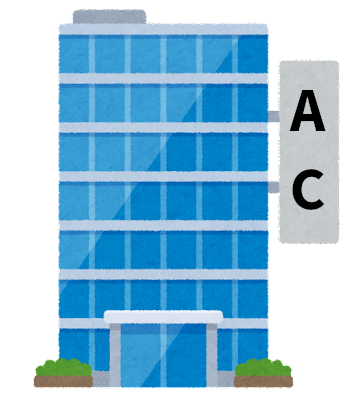
\includegraphics[width=0.15\textwidth]{images/ac_games.png}};
    \node<2->[below=0cm of acgames] (acgames-name) {AC-Games};
    
    \node<3->[left=3cm of acgames] (nutzer) {
\includegraphics[width=0.15\textwidth]{images/game_friends.png}};
    \node<3->[below=0cm of nutzer] (nutzer-name) {Nutzer:innen};
    
    \draw<2->[-stealth] (walter) -- node[below] {CEO}  (acgames);
    \draw<3->[-stealth] (nutzer) -- node[below] (geld) {Geld} (acgames);
  \end{tikzpicture} 
\end{frame}

\begin{frame}{Finanzkrise}
  \centering
  
  \note[item]<1-> {Gibt jetzt Probleme}
  \note[item]<2-> {Finanzkrise vor 10 Jahren (zu dem Zeitpunkt) \begin{itemize}
      \item Langsam sinken Einnahmen \begin{itemize}
          \item App Stores (KLICK) $\Rightarrow$ Spieleportal von Entwicklern kaum genutzt
          \item Werbeaufträge gehen zurück
          \item Weniger In-Game Käufe
      \end{itemize}
      \item seit 3 Jahren nicht mehr genug
      \item kann Mitarbeiter nicht mehr bezahlen
  \end{itemize}}
  \note[item]<4-> {AC-Games droht Bankrott}
  
  \begin{tikzpicture}
    \node (walter) {
\includegraphics[width=0.15\textwidth]{images/walter.png}};
    \node[below=0mm of walter] (walter-name) {Walter};
    
    \node[left=3cm of walter] (acgames) {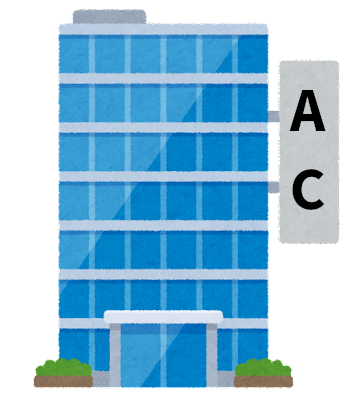
\includegraphics[width=0.15\textwidth]{images/ac_games.png}};
    \node[below=0cm of acgames] (acgames-name) {AC-Games};
    
    \node[left=3cm of acgames] (nutzer) {
\includegraphics[width=0.15\textwidth]{images/game_friends.png}};
    \node[below=0cm of nutzer] (nutzer-name) {Nutzer:innen};
    
    
    \draw<1-3>[-stealth] (walter) -- node[below] (ceo) {CEO}  (acgames);
    \draw<1>[-stealth] (nutzer) -- node[below] (geld) {Geld} (acgames);
    
    % Finanzkrise 2
    
    \draw<2->[-stealth, red] (nutzer) -- node[below] (geld) {Geld} (acgames);
    
    \node<2->[above=1cm of geld] (finanzkrise) {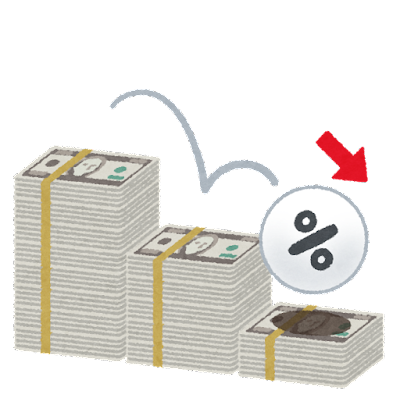
\includegraphics[width=0.12\textwidth]{images/money_down.png}};
    \node<2->[below=0cm of finanzkrise] (finanzkrise-name) {Finanzkrise};
    \draw<2->[dotted, red] (finanzkrise-name) -- (geld);
    
    % App Stores machen obsolet 3
    
    \node<3->[below=0.5cm of geld] (apps) {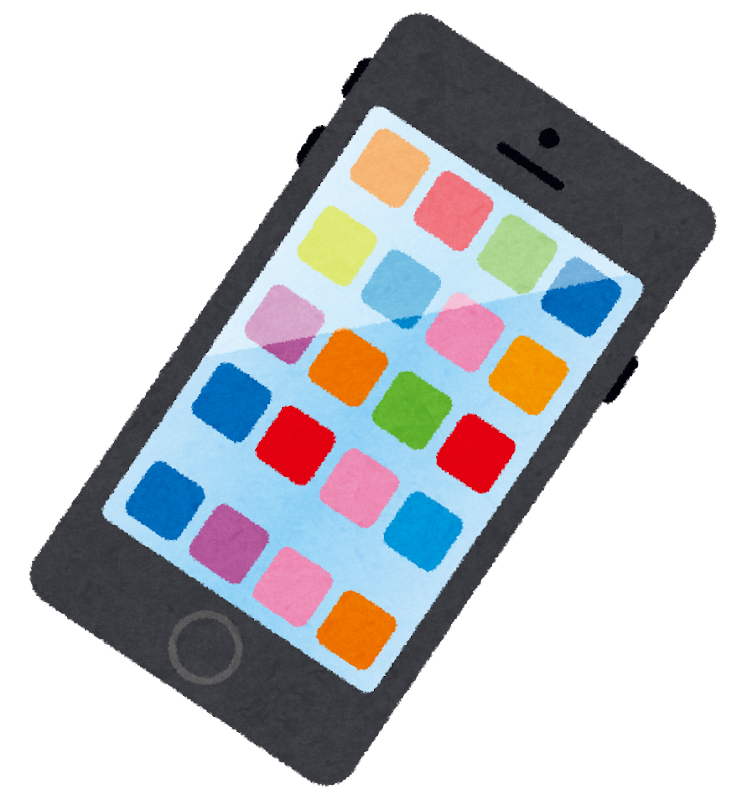
\includegraphics[width=0.10\textwidth]{images/smartphone.png}};
    \node<3->[below=0cm of apps] (apps-name) {App-Stores};
    \draw<3->[dotted, red] (apps) -- (geld);
    
    % Bankrott
    
    \node<4->[left=2.7cm of walter] (batsu) {
\includegraphics[width=0.2\textwidth]{images/batsu.png}};
    \draw<4->[-stealth, red] ([yshift=1mm]acgames.east) -- node[above] {Droht Bankrott} ([yshift=1mm]walter.west);
    \draw<4->[-stealth] ([yshift=-1mm]walter.west) -- node[below] (ceo) {CEO} ([yshift=-1mm]acgames.east);
  \end{tikzpicture} 
\end{frame}
\begin{frame}{Ein Angebot}
  \centering
  
  \note<1->[item]{Nachgrübeln was zu tun}
  \note<1->[item]{Plötzlich ein Angebot}
  \note<2->[item]{Firma "Data Broker GmbH" will Firma übernehmen \begin{itemize}
      \item Bietet Geld. (KLICK) VIEL Geld
  \end{itemize}}
  \note<4->[item]{Mitarbeiter fragen sich: Woher der hohe Preis?}
  \note<4->[item]{Gesammelte Daten sind nur für Transaktionen Wichtige}
  
  \begin{tikzpicture}
    \node<1-3> (walter) {
\includegraphics[width=0.15\textwidth]{images/walter.png}};
    \node<1-3>[below=0mm of walter] (walter-name) {Walter};
    
    \node<2-3>[right=4cm of walter] (databroker) {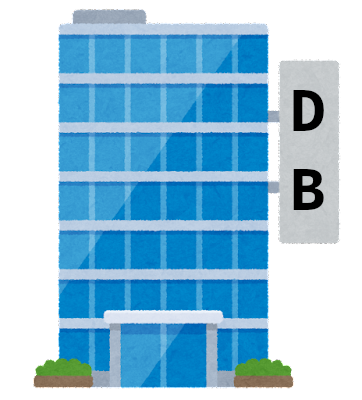
\includegraphics[width=0.15\textwidth]{images/data_broker.png}};
    \node<2-3>[below=0cm of databroker] (databroker-name) {Data Broker GmbH};
    
    % Data Broker kommt
    
    \draw<2-3>[stealth-] ([yshift=1mm]databroker.west) -- node[above] (acgames-name) {AC-Games}  ([yshift=1mm]walter.east);
    \node<2-3>[above=0cm of acgames-name] (acgames) {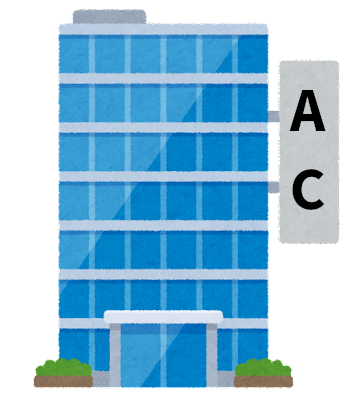
\includegraphics[width=0.075\textwidth]{images/ac_games.png}};
    \draw<2>[stealth-] ([yshift=-1mm]walter.east) -- node[below] {
\includegraphics[width=0.075\textwidth]{images/dollar_bill.png}}  ([yshift=-1mm]databroker.west);
    
    % MORE MONEY
    
    \draw<3>[stealth-] ([yshift=-1mm]walter.east) -- node[below] {
\includegraphics[width=0.1\textwidth]{images/money_bag_dollar.png}} ([yshift=-1mm]databroker.west);
    
    % Warum so viel geld?
    
    \node<4-> (typ) {
\includegraphics[width=0.45\textwidth]{images/pose_shinpai_fukidashi_man.png}};
    \node<4->[above=0cm of typ.center] (money) {
\includegraphics[width=0.18\textwidth]{images/money_bag_dollar.png}};
    
  \end{tikzpicture} 
\end{frame}

\begin{frame}{Ein Angebot}
  \centering
  
  \note[item] {Pro \begin{itemize}
      \item Firma bleibt relativ sicher bestehen
      \item Spieler und ihr Investment werden nicht im Stich gelassen
  \end{itemize}}
  \note[item]{Contra \begin{itemize}
      \item Daten in der Hand von Datenhändler \begin{itemize}
          \item Hoher Preis wird wohl seinen Grund haben
          \item Wahrscheinlich nicht aus reiner Wohltat
      \end{itemize}
  \end{itemize}}
  \note[item]{Alternativen \begin{itemize}
      \item Crowdfunding
      \item Vielleicht an dieser Stelle zu spät, aber hätte sich ein anderes Produkt überlegen können \begin{itemize}
          \item Haben ja schon Jahre vorher gemerkt, dass es mit ihrem Produkt abwärtsgeht
      \end{itemize}
  \end{itemize}}
  
  \Large
  Sollte Walter AC-Games an Data Broker verkaufen?\\
  Wenn nein, gibt es eine Alternative?
  
  
\includegraphics[width=0.425\textwidth]{images/discussion.png}
\end{frame}

\begin{frame}{Ein Angebot}
  \centering
  
  \note[item] {Pro \begin{itemize}
    \item Offensichtlich: Firma soll überleben
  \end{itemize}}
  \note[item]{Contra \begin{itemize}
    \item Finanzkrise ist ja nicht einziger Grund
    \item App Stores etc. bieten scheinbar besseren Service
    \item In-Game Käufe lassen nach $\Rightarrow$ hört sich eher nach Problem mit Produkt selbst an
  \end{itemize}}
  
  \Large
  Wie bewertet ihr, dass AC-Games trotz finanzieller Schwierigkeiten ihr Portal weiter betreiben wollen? 
  
  
\includegraphics[width=0.425\textwidth]{images/discussion.png}
\end{frame}


\begin{frame}{Übernahme}
    
\end{frame}  

\begin{frame}[t,standout]
\Large
Clever Last Words to Stimulate Discussion
\end{frame}

\nocite{kees_faites_2017}
\nocite{lee_ethical_2016}
\nocite{zankl_international_2014}

\begin{frame}{Literatur}
\printbibliography[heading=none]
\end{frame}


\end{document}
